\documentclass[12pt,a4paper]{article}

% ── Encoding & Language ───────────────────────────────────────────
\usepackage[utf8]{inputenc}
\usepackage[T1]{fontenc}
\usepackage[english]{babel}
\usepackage{csquotes}

% ── Geometry & Spacing ────────────────────────────────────────────
\usepackage[top=3cm,bottom=2.5cm,left=2.5cm,right=2.5cm]{geometry}
\usepackage{setspace}
\onehalfspacing

% ── Graphics & Figures ────────────────────────────────────────────
\usepackage{graphicx}
\usepackage{tikz}
\usetikzlibrary{shapes.geometric, arrows.meta, positioning, fit, backgrounds}
\usepackage{float}

% ── Tables & Lists ────────────────────────────────────────────────
\usepackage{booktabs}
\usepackage{longtable}
\usepackage{array}
\usepackage{multirow}
\usepackage{enumitem}
\setlist{nosep,leftmargin=*}

% ── Maths ─────────────────────────────────────────────────────────
\usepackage{amsmath}
\usepackage{amssymb}
\usepackage{siunitx}
\sisetup{detect-all}

% ── Hyperlinks & Metadata ─────────────────────────────────────────
\usepackage[colorlinks=true,linkcolor=blue,citecolor=blue,urlcolor=blue]{hyperref}
\usepackage{url}

% ── Captions ──────────────────────────────────────────────────────
\usepackage{caption}
\usepackage{subcaption}

% ── Title Metadata ────────────────────────────────────────────────
\title{
  \vspace{-2cm}
  \textbf{Conceptual Design Proposal}\\[0.3cm]
  \large SDR-Based Monitoring System for Electric Field Exposure\\
  in High-Density IoT Indoor Environments
}
\author{
  \small
  Control and Digital Signal Processing Group (GCPDS)\\
  Universidad Nacional de Colombia --- Manizales Campus\\
  \vspace{0.2cm}\\
  Universidad de Caldas
}
\date{\small \today}

\begin{document}

\maketitle
\thispagestyle{empty}

% ── Abstract ──────────────────────────────────────────────────────
\begin{abstract}
\noindent
This document presents the conceptual design of an IoT platform based on Software-Defined Radio (SDR) for monitoring human exposure to electric fields in indoor environments with a high density of IoT devices. The proposed architecture consists of five main components: SDR hardware, a real-time acquisition engine in C, digital signal processing and business logic in Python, a TimescaleDB time-series database, and a reactive web interface. The system employs machine learning techniques for adaptive thresholding, cooperative spectrum sensing, and geostatistical interpolation (Kriging) for generating electromagnetic exposure heatmaps, all in compliance with ICNIRP and ITU-T K.52 standards. The hardware bill of materials (BOM), the RF signal chain, and the project timeline are included.
\end{abstract}

\vspace{1cm}
{\small
\noindent\textbf{Keywords:} SDR, IoT, electromagnetic exposure, Kriging, machine learning, USRP B210, Jetson Orin, heatmaps.
}

\newpage
\tableofcontents
\newpage

% ═══════════════════════════════════════════════════════════════════════
% 1. INTRODUCTION
% ═══════════════════════════════════════════════════════════════════════
\section{Introduction}

\subsection{Problem Statement}

The proliferation of IoT devices in enclosed work environments (offices, factories, data centers) raises growing concern about cumulative exposure to electric fields. Traditional spectrum analyzers are expensive, bulky, and impractical for dense or mobile indoor studies. Software-Defined Radio (SDR) emerges as a lower-cost, more flexible alternative, albeit with limitations in dynamic range, ADC/DAC behaviour, and usable frequency band.

The system must operate in the proposed range of \qtyrange{700}{3500}{\MHz}, covering the main IoT and telecommunications bands (LTE, WiFi 2.4~GHz, ISM). Indoor environments require numerous fast measurements to identify high-radiation zones and compare them against exposure standards.

\subsection{Rationale}

Static thresholding proves insufficient in noisy, dynamic IoT environments. The proposal incorporates adaptive thresholding based on machine learning and cooperative sensing. Electric field exposure maps allow correlating device density, frequency usage, and exposure levels, constituting both a scientific and a regulatory tool.

\subsection{Research Question}

\noindent
\textit{How does IoT device density influence electric field exposure levels in enclosed environments, and what impact might such exposure have on workers’ health, using an SDR-based monitoring system and advanced machine learning techniques for detection and analysis?}

\subsection{Objectives}

\paragraph{General Objective}
Develop a system for assessing human exposure levels to electric fields, based on SDR and machine learning techniques, capable of measuring radiation density in indoor environments with high IoT device occupancy.

\paragraph{Specific Objectives}
\begin{enumerate}[label=SO\arabic*:,leftmargin=2.5em]
  \item Design and build an SDR measurement module for spectral monitoring of high-density IoT networks in indoor spaces, using spectrum sensing techniques.
  \item Develop thresholding algorithms and cooperative processes based on machine learning methods to handle measurement variability in indoor environments with high interference.
  \item Generate spatial electric field maps using advanced measurement and data analysis techniques to assess compliance with human exposure regulations.
\end{enumerate}

% ═══════════════════════════════════════════════════════════════════════
% 2. SYSTEM ARCHITECTURE
% ═══════════════════════════════════════════════════════════════════════
\section{System Architecture}

\subsection{Overview}

The system comprises five main modules working together to capture, process, store, and visualise electric field exposure data. The architecture is designed under the principles of real-time processing, low latency, and component decoupling, allowing each module to evolve independently.

\begin{figure}[H]
\centering
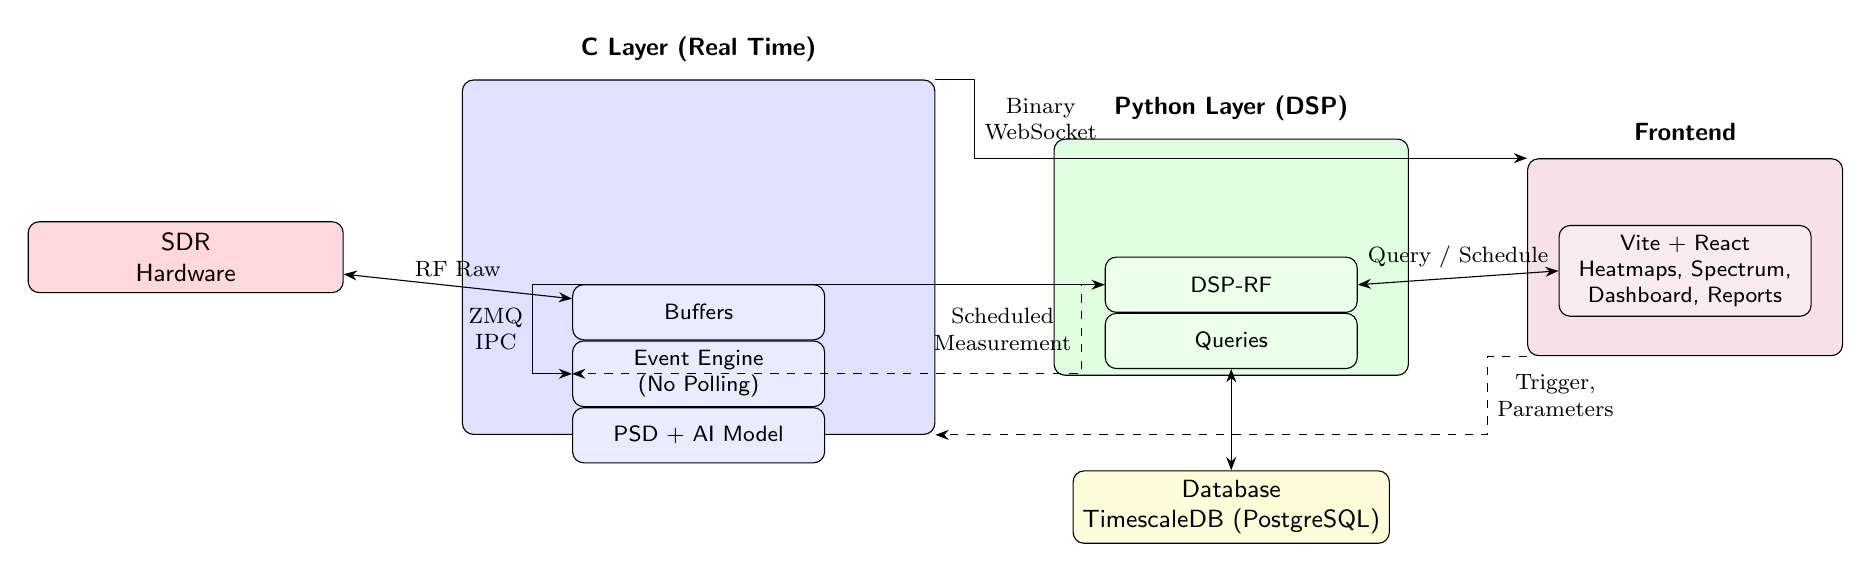
\begin{tikzpicture}[
  node distance=1.2cm and 1.5cm,
  box/.style={rectangle, draw=black, rounded corners, minimum width=4cm, minimum height=0.9cm, align=center, font=\small\sffamily},
  sbox/.style={box, minimum width=3.2cm, minimum height=0.7cm, font=\footnotesize\sffamily},
  >={Stealth[scale=0.8]},
  line/.style={draw, ->, >=Stealth},
  doubleline/.style={draw, <->, >=Stealth},
]
  % ── SDR ────────────────────────────────────
  \node[box, fill=red!15] (sdr) {SDR\\Hardware};

  % ── C Layer ────────────────────────────────
  \node[box, fill=blue!12, right=of sdr, minimum height=4.5cm, minimum width=6cm] (clayer) {};
  \node[font=\small\sffamily\bfseries, above=0.1cm of clayer.north] {C Layer (Real Time)};
  \node[sbox, fill=blue!8, above=1.2cm of clayer.south] (buffers) {Buffers};
  \node[sbox, fill=blue!8, below=0.0cm of buffers] (engine) {Event Engine\\(No Polling)};
  \node[sbox, fill=blue!8, below=0.0cm of engine] (psd) {PSD + AI Model};

  % ── Python Layer ───────────────────────────
  \node[box, fill=green!12, right=of clayer, minimum height=3cm, minimum width=4.5cm] (python) {};
  \node[font=\small\sffamily\bfseries, above=0.1cm of python.north] {Python Layer (DSP)};
  \node[sbox, fill=green!8, above=0.8cm of python.south] (dsp) {DSP-RF};
  \node[sbox, fill=green!8, below=0.0cm of dsp] (queries) {Queries};

  % ── Database ───────────────────────────────
  \node[box, fill=yellow!15, below=of python, minimum width=4cm] (db) {Database\\TimescaleDB (PostgreSQL)};

  % ── Frontend ───────────────────────────────
  \node[box, fill=purple!12, right=of python, minimum height=2.5cm, minimum width=4cm] (frontend) {};
  \node[font=\small\sffamily\bfseries, above=0.1cm of frontend.north] {Frontend};
  \node[sbox, fill=purple!8, above=0.5cm of frontend.south] (react) {Vite + React\\Heatmaps, Spectrum,\\ Dashboard, Reports};

  % ── Connections ────────────────────────────
  \draw[doubleline] (sdr) -- node[above,font=\footnotesize] {RF Raw} (buffers);
  \draw[doubleline] (engine.west) -- ++(-0.5,0) |- node[pos=0.25,left,font=\footnotesize,align=center] {ZMQ\\IPC} (dsp.west);
  \draw[line, dashed] (dsp.west) -- ++(-0.3,0) |- node[pos=0.25,left,font=\footnotesize,align=center] {Scheduled\\Measurement} (engine.west);
  \draw[line] (clayer.north east) -- ++(0.5,0) |- node[pos=0.25,right,font=\footnotesize,align=center] {Binary\\WebSocket} (frontend.north west);
  \draw[line, dashed] (frontend.south west) -- ++(-0.5,0) |- node[pos=0.25,right,font=\footnotesize,align=center] {Trigger,\\Parameters} (clayer.south east);
  \draw[doubleline] (dsp.east) -- node[above,font=\footnotesize] {Query / Schedule} (react.west);
  \draw[doubleline] (queries.south) -- (db.north);

\end{tikzpicture}
\caption{Conceptual diagram of the 5-component architecture. Solid lines represent primary data flows; dashed lines represent control commands.}
\label{fig:arch}
\end{figure}

\subsection{Component 1: SDR (Software-Defined Radio)}

\textbf{Role:} External RF capture device.

The SDR is the entry point for electromagnetic signals into the system. It captures raw RF samples, covering the range of \qtyrange{698}{6000}{\MHz} with an instantaneous bandwidth of up to \qty{56}{\MHz}. The hardware selected for the prototype is the Ettus Research USRP B210, which offers a 2$\times$2 MIMO architecture with 12-bit ADC/DAC resolution and a USB~3.0 interface.

The connection to the system is bidirectional: raw samples flow into the C-layer buffers, while configuration commands (frequency, gain, sampling rate) can be sent back to the SDR.

\subsection{Component 2: C Layer --- Real-Time Engine}

\textbf{Role:} High-performance signal acquisition and preprocessing.

The C layer is the real-time processing core of the system. It is implemented in C11 and runs directly on the host hardware (not in a container), as it requires direct access to the SDR's USB peripherals. It consists of three submodules:

\paragraph{Buffers}
Act as a bridge between the SDR hardware and internal processing. They receive raw samples from the SDR in bidirectional mode and deliver them to the event engine, ensuring continuous flow without data loss.

\paragraph{Event Engine (No Polling)}
Event-driven architecture that explicitly avoids polling to minimise CPU usage and latency in real-time signal processing. It reacts to data arrival from the buffers and:
\begin{itemize}
  \item Sends data and events to the Python layer via \textbf{ZMQ over IPC} (inter-process communication) for high-level processing.
  \item Receives control commands from Python (\textit{scheduled measurement}).
  \item Streams binary spectral data directly to the web frontend via \textbf{WebSocket} (Libwebsockets), bypassing Python for latency-sensitive flows.
  \item Receives control commands from the frontend (\textit{trigger}, \textit{parameter changes}).
\end{itemize}

\paragraph{PSD (Power Spectral Density) + AI Model}
Power Spectral Density analysis module embedded directly in the C layer. It incorporates an artificial intelligence model for spectral analysis and anomaly detection, operating close to the data source for low-latency inference. The model is trained for adaptive thresholding and false-alarm reduction in high-interference environments.

\subsection{Component 3: Python Layer --- DSP and Business Logic}

\textbf{Role:} High-level digital signal processing, data orchestration, and business logic.

The Python layer leverages the scientific ecosystem (NumPy, SciPy) for RF processing that does not require the minimal latency of the C layer. It consists of two submodules:

\paragraph{DSP-RF}
Digital Signal Processing module focused on RF. It receives events and data from the C layer via ZMQ IPC, applies advanced spectral analysis algorithms, and sends scheduled measurement commands back to the C layer. It also communicates bidirectionally with the frontend for \textit{query} and \textit{scheduling} operations for measurement campaigns.

\paragraph{Queries}
Data access layer that manages all persistence. It interacts bidirectionally with the database to store measurements, algorithm results, configurations, campaigns, and reports. It implements the business logic for scientific traceability: each measurement is linked to its acquisition configuration, AI model, campaign, and spatial location.

\subsection{Component 4: Database --- TimescaleDB}

\textbf{Role:} Persistent time-series storage with analytical query capabilities.

TimescaleDB (an extension on top of PostgreSQL 16) provides:
\begin{itemize}
  \item Efficient time-series storage (timestamped spectral measurements).
  \item Native compression and automatic partitioning (hypertables) for high-frequency data.
  \item Full relational model for metadata: sensors, antennas, configurations, campaigns, algorithms, thresholds, alerts, users, and compliance reports.
  \item End-to-end traceability from raw capture to exportable report.
\end{itemize}

\subsection{Component 5: Frontend --- User Interface}

\textbf{Role:} Reactive visualisation for monitoring, control, and querying.

Single-page application (SPA) built with Vite + React + TypeScript, designed with Material UI (dark theme). The main visualisation components include:

\begin{itemize}
  \item \textbf{Live Spectrum:} Waterfall plot and real-time FFT, fed directly by the binary WebSocket stream from the C layer (Plotly.js).
  \item \textbf{IoT Heatmap:} Electric field exposure map overlaid on floor plans, generated via Kriging interpolation from spatial measurements. Supports grid overlay and measurement point placement.
  \item \textbf{Sensor Status:} Health monitoring, telemetry, and connectivity of deployed SDR sensors.
  \item \textbf{Campaign Management:} Scheduling of measurement campaigns with sensor assignment, frequency ranges, resolution, and intervals.
  \item \textbf{Exportable Reports:} Automatic generation of regulatory compliance reports (ICNIRP, ITU-T K.52) with result caching.
  \item \textbf{Configuration Panel:} Service status, system parameters, and access control.
\end{itemize}

% ═══════════════════════════════════════════════════════════════════════
% 3. COMMUNICATION CHANNELS
% ═══════════════════════════════════════════════════════════════════════
\section{Communication Channels}

Table~\ref{tab:channels} summarises the communication channels between components, the protocol used, and the data flow direction.

\begin{table}[H]
\centering
\caption{System communication channels}
\label{tab:channels}
\begin{tabular}{@{}llll@{}}
\toprule
\textbf{Source} & \textbf{Destination} & \textbf{Protocol} & \textbf{Direction} \\
\midrule
SDR & Buffers (C) & Raw RF samples & Bidirectional \\
Buffers (C) & Event Engine (C) & Internal flow & Internal \\
Event Engine (C) & DSP-RF (Python) & ZMQ over IPC & Bidirectional \\
DSP-RF (Python) & Event Engine (C) & Scheduled measurement & Python $\to$ C \\
C Layer & Frontend (React) & Binary WebSocket & C $\to$ Frontend \\
Frontend (React) & C Layer & WebSocket (control) & Frontend $\to$ C \\
DSP-RF (Python) & Frontend (React) & HTTP (REST) & Bidirectional \\
Queries (Python) & Database & SQL & Bidirectional \\
\bottomrule
\end{tabular}
\end{table}

\subsection{Communication Design Decisions}

\begin{description}
  \item[ZMQ over IPC] ZeroMQ with inter-process communication (IPC) provides low-latency messaging between the C and Python processes co-located on the same host, eliminating network stack overhead.
  \item[Direct binary WebSocket] The spectral data stream is transmitted directly from the C layer to the browser without going through Python. This minimises latency for real-time visualisations (waterfall, FFT) that require a high refresh rate.
  \item[HTTP REST for queries] Query and scheduling operations between the frontend and the Python backend use HTTP/REST, suitable for transactional operations that do not require continuous streaming.
\end{description}

% ═══════════════════════════════════════════════════════════════════════
% 4. HARDWARE BILL OF MATERIALS
% ═══════════════════════════════════════════════════════════════════════
\section{Hardware Bill of Materials (BOM)}

The monitoring system is portable and self-contained, designed to capture, process, and visualise RF signals in the range of \qtyrange{698}{6000}{\MHz}. Each hardware component is detailed below with its role, specifications, supplier, and cost.

\subsection{Cost Summary}

\begin{table}[H]
\centering
\caption{Hardware cost summary}
\label{tab:cost}
\begin{tabular}{@{}lrr@{}}
\toprule
\textbf{Component} & \textbf{Unit Price (USD)} & \textbf{Imported Price (USD)} \\
\midrule
USRP B210 & \$2,200.00 & \$2,860.00 \\
Antenna 698--2700 MHz & \$200.00   & \$260.00   \\
Preselection Filters ($\times$2) & \$200.00   & \$260.00   \\
Jetson Orin Nano Super & \$300.00   & \$390.00   \\
7'' Touchscreen & \$60.00    & \$78.00    \\
Custom Enclosure & \$100.00   & \$130.00   \\
\midrule
\textbf{TOTAL} & \textbf{\$3,060.00} & \textbf{\$3,978.00} \\
\bottomrule
\end{tabular}
\end{table}

\subsection{Per-Component Specifications}

\subsubsection{SDR --- Ettus Research USRP B210}

\textbf{Role:} Main RF front-end. Broadband spectrum capture and transmission via USB 3.0 to the computing module.

\begin{table}[H]
\centering
\caption{USRP B210 specifications}
\begin{tabular}{@{}ll@{}}
\toprule
\textbf{Parameter} & \textbf{Value} \\
\midrule
Model / Part & USRP B210 (Kit, UB210-KIT) \\
Supplier & Ettus Research (National Instruments) \\
Frequency range & \qtyrange{70}{6000}{\MHz} continuous \\
RF bandwidth & Up to \qty{56}{\MHz} instantaneous \\
Architecture & 2$\times$2 MIMO (2 TX, 2 RX) \\
ADC/DAC & 12 bits \\
Host interface & USB 3.0 \\
FPGA & Xilinx Spartan-6 XC6SLX150 \\
Noise figure & $\approx$\qty{8}{\dB} \\
Impedance & \qty{50}{\ohm} \\
RF connectors & 4 SMA (RX/TX per channel) \\
Supported software & GNU Radio, UHD, MATLAB, LabVIEW \\
\bottomrule
\end{tabular}
\end{table}

\subsubsection{Computing Module --- NVIDIA Jetson Orin Nano Super}

\textbf{Role:} Central processing unit for AI inference, signal processing, system control, and display output.

\begin{table}[H]
\centering
\caption{Jetson Orin Nano Super specifications}
\begin{tabular}{@{}ll@{}}
\toprule
\textbf{Parameter} & \textbf{Value} \\
\midrule
Model & Jetson Orin Nano Super Developer Kit (945-13766-0005-000) \\
AI performance & Up to 67 TOPS \\
GPU & NVIDIA Ampere, 1024 CUDA cores \\
CPU & 6-core ARM Cortex-A78AE \\
RAM & 8~GB LPDDR5, 102~GB/s bandwidth \\
Storage & 2$\times$ M.2 Key M (NVMe SSD) \\
USB & 4$\times$ USB 3.2 Gen 2 Type-A, 1$\times$ USB-C \\
Video & DisplayPort 1.2 (HDMI via adapter) \\
Connectivity & Wi-Fi (M.2 Key E), Gigabit Ethernet \\
GPIO & 40-pin header \\
Operating system & JetPack (Ubuntu Linux) \\
AI support & TensorRT, PyTorch, ROS 2, GNU Radio \\
\bottomrule
\end{tabular}
\end{table}

\subsubsection{Omnidirectional Antenna --- L-com LCANOM1075}

\textbf{Role:} Main RF signal capture element in the \qtyrange{698}{2700}{\MHz} range.

\begin{table}[H]
\centering
\caption{Antenna specifications}
\begin{tabular}{@{}ll@{}}
\toprule
\textbf{Parameter} & \textbf{Value} \\
\midrule
Model & LCANOM1075 \\
Manufacturer & L-com \\
Frequency range & \qtyrange{698}{2700}{\MHz} \\
Gain & 6.5~dBi \\
Radiation pattern & Omnidirectional \\
Polarisation & Vertical \\
Connector & SMA Male (spring, \qty{5.5}{\mm}) \\
Radome & Fibreglass, black \\
Impedance & \qty{50}{\ohm} \\
VSWR & $\leq$ 2.0 (typical) \\
\bottomrule
\end{tabular}
\end{table}

\subsubsection{Preselection Filters --- Mini-Circuits}

\textbf{Role:} Bandpass filtering between the antenna and the USRP B210. They suppress out-of-band interference before digitisation, improving sensitivity and reducing intermodulation. Two filters are used, one per RX channel of the USRP B210.

\begin{table}[H]
\centering
\caption{Filter 1 --- VBFZ-925-S+}
\begin{tabular}{@{}ll@{}}
\toprule
\textbf{Parameter} & \textbf{Value} \\
\midrule
Model & VBFZ-925-S+ \\
Manufacturer & Mini-Circuits \\
Type & Connectorised bandpass filter \\
Passband & \qtyrange{800}{1050}{\MHz} \\
Connector & SMA \\
Impedance & \qty{50}{\ohm} \\
Spectral coverage & GSM 850, GSM 900, LTE B5/B8/B20 \\
\bottomrule
\end{tabular}
\end{table}

\begin{table}[H]
\centering
\caption{Filter 2 --- BPF-A1340+}
\begin{tabular}{@{}ll@{}}
\toprule
\textbf{Parameter} & \textbf{Value} \\
\midrule
Model & BPF-A1340+ \\
Manufacturer & Mini-Circuits \\
Type & LC bandpass filter \\
Passband & \qtyrange{1000}{1800}{\MHz} \\
Connector & SMA \\
Impedance & \qty{50}{\ohm} \\
Spectral coverage & GPS L1 (1575 MHz), DCS 1800, LTE B1/B3/B4/B10 \\
\bottomrule
\end{tabular}
\end{table}

The combination of both filters provides preselection in the \qtyrange{800}{1800}{\MHz} range, enabling simultaneous monitoring of two independent bands.

\subsubsection{Touchscreen --- Waveshare 7'' HDMI LCD (C)}

\textbf{Role:} Touch-based user interface for spectrum display, heatmaps, dashboards, and system status.

\begin{table}[H]
\centering
\caption{Display specifications}
\begin{tabular}{@{}ll@{}}
\toprule
\textbf{Parameter} & \textbf{Value} \\
\midrule
Model & Waveshare 7'' HDMI LCD (C), Rev 4.1 \\
Size & 7~inches \\
Panel type & IPS \\
Resolution & 1024 $\times$ 600 \\
Touch & Capacitive, 5-point \\
Video interface & HDMI \\
Touch interface & USB Micro-B (HID) \\
Supported systems & Ubuntu, Raspbian, Windows, JetPack \\
\bottomrule
\end{tabular}
\end{table}

\subsubsection{Custom Enclosure}

\textbf{Role:} Mechanical container for all components. Provides physical protection, cable management, and mounting points for the antenna and display.

\textbf{Design requirements:}
\begin{itemize}
  \item Accommodate USRP B210 PCB, Jetson Orin Nano, and 7~inch display.
  \item External antenna mounting port (SMA bulkhead).
  \item Access to USB 3.0 port for USRP B210 connection.
  \item Ventilation for thermal dissipation (Jetson $\approx$ \qty{15}{\W}).
  \item Display window ($\approx$ \qtyproduct{165 x 100}{\mm} visible area).
  \item Portable form factor, rugged instrument-case style.
\end{itemize}

\subsection{RF Signal Chain}

Figure~\ref{fig:signalchain} shows the RF signal flow from the antenna to the display.

\begin{figure}[H]
\centering
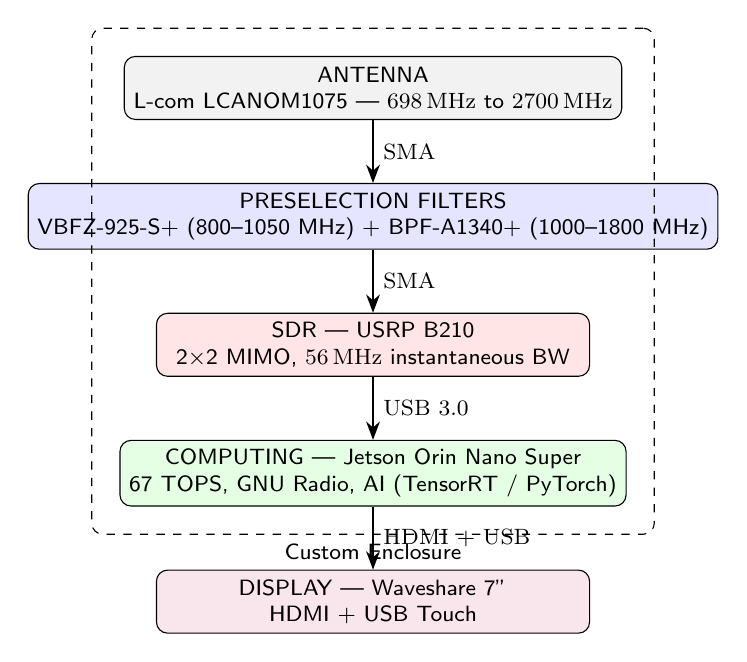
\begin{tikzpicture}[
  node distance=0.8cm,
  block/.style={rectangle, draw, rounded corners, minimum width=5.5cm, minimum height=0.8cm, align=center, font=\footnotesize\sffamily},
  >={Stealth[]},
]
  \node[block, fill=gray!10] (ant) {ANTENNA\\L-com LCANOM1075 --- \qtyrange{698}{2700}{\MHz}};
  \node[block, fill=blue!10, below=of ant] (filtros) {PRESELECTION FILTERS\\VBFZ-925-S+ (800--1050 MHz) + BPF-A1340+ (1000--1800 MHz)};
  \node[block, fill=red!10, below=of filtros] (usrp) {SDR --- USRP B210\\2$\times$2 MIMO, \qty{56}{\MHz} instantaneous BW};
  \node[block, fill=green!10, below=of usrp] (jetson) {COMPUTING --- Jetson Orin Nano Super\\67 TOPS, GNU Radio, AI (TensorRT / PyTorch)};
  \node[block, fill=purple!10, below=of jetson] (display) {DISPLAY --- Waveshare 7''\\HDMI + USB Touch};
  \node[draw, dashed, rounded corners, fit=(ant)(jetson), inner sep=10pt, label={[font=\footnotesize\sffamily]below:Custom Enclosure}] {};

  \draw[->,thick] (ant) -- node[right,font=\footnotesize] {SMA} (filtros);
  \draw[->,thick] (filtros) -- node[right,font=\footnotesize] {SMA} (usrp);
  \draw[->,thick] (usrp) -- node[right,font=\footnotesize] {USB 3.0} (jetson);
  \draw[->,thick] (jetson) -- node[right,font=\footnotesize] {HDMI + USB} (display);
\end{tikzpicture}
\caption{RF signal chain: from antenna to display.}
\label{fig:signalchain}
\end{figure}

% ═══════════════════════════════════════════════════════════════════════
% 5. AI AND INTERPOLATION STRATEGY
% ═══════════════════════════════════════════════════════════════════════
\section{AI and Interpolation Strategy}

\subsection{Adaptive Thresholding and Cooperative Sensing}

The traditional static thresholding system is unsuitable for IoT environments with high device density, where noise and interference levels vary significantly. The proposal incorporates:

\begin{itemize}
  \item \textbf{Autoencoders} for feature extraction and dimensionality reduction in raw spectral data. They enable identifying interference patterns characteristic of IoT environments and distinguishing them from anomalies requiring attention.
  \item \textbf{Two-level thresholding} inspired by cooperative communication systems (such as 5G): a fast first threshold for coarse detection and a refined second threshold, cooperatively validated across multiple sweeps or frequencies, for false-alarm reduction.
  \item \textbf{AI model embedded in the C layer} (PSD module) operating with low-latency inference, close to the data source, without requiring transfer to the Python backend for real-time decisions.
\end{itemize}

\subsection{Kriging Interpolation}

For generating spatial electric field exposure maps, Kriging interpolation is employed, a geostatistical method that:

\begin{itemize}
  \item Estimates values at unsampled locations from a discrete set of measurement points with geographic coordinates (latitude, longitude).
  \item Provides not only the point estimate but also the estimation error variance, enabling assessment of the generated map's reliability.
  \item Reduces the number of required measurement points through intelligent selective sampling, preserving map quality and optimising the characterisation time of an indoor environment.
\end{itemize}

% ═══════════════════════════════════════════════════════════════════════
% 6. DATA MODEL CONCEPT
% ═══════════════════════════════════════════════════════════════════════
\section{Conceptual Data Model}

The data model is designed to ensure complete scientific traceability: every measurement can be traced back to its acquisition configuration, sensor, campaign, AI model, and location.

\begin{figure}[H]
\centering
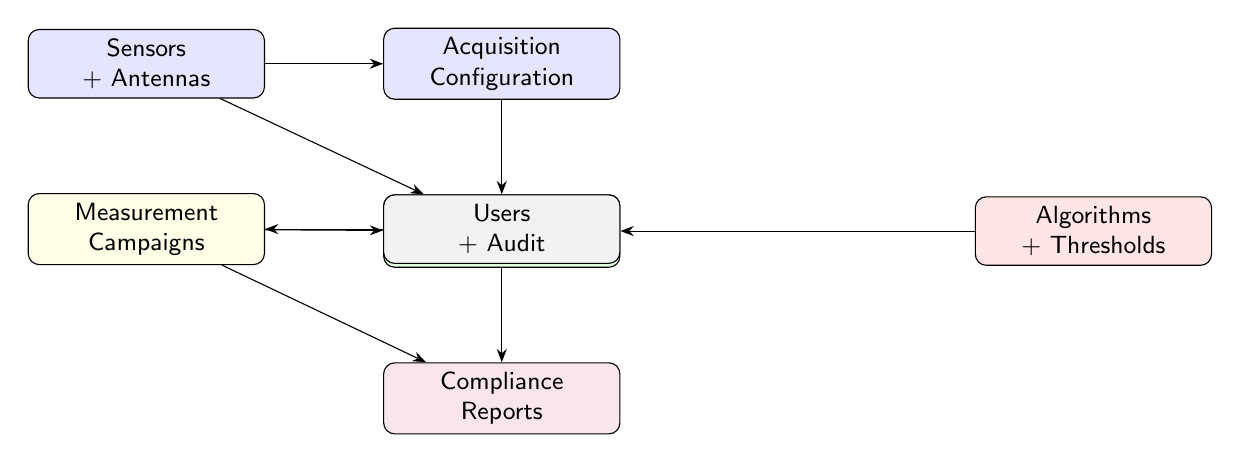
\begin{tikzpicture}[
  node distance=1.2cm and 1.5cm,
  entity/.style={rectangle, draw, rounded corners, minimum width=3cm, minimum height=0.7cm, align=center, font=\small\sffamily},
  rel/.style={draw, ->, >=Stealth},
]
  \node[entity, fill=blue!10] (sensor) {Sensors\\+ Antennas};
  \node[entity, fill=blue!10, right=of sensor] (config) {Acquisition\\Configuration};
  \node[entity, fill=green!10, below=of config] (data) {Measurements\\(Sensor Data)};
  \node[entity, fill=yellow!10, below=of sensor] (campaign) {Measurement\\Campaigns};
  \node[entity, fill=red!10, right=4.5cm of data] (algo) {Algorithms\\+ Thresholds};
  \node[entity, fill=purple!10, below=of data] (report) {Compliance\\Reports};
  \node[entity, fill=gray!10, right=of campaign] (user) {Users\\+ Audit};

  \draw[rel] (sensor) -- (config);
  \draw[rel] (sensor) -- (data);
  \draw[rel] (config) -- (data);
  \draw[rel] (campaign) -- (data);
  \draw[rel] (algo) -- (data);
  \draw[rel] (data) -- (report);
  \draw[rel] (campaign) -- (report);
  \draw[rel] (user) -- (campaign);
\end{tikzpicture}
\caption{Conceptual data model: traceability from sensor to compliance report.}
\label{fig:datamodel}
\end{figure}

The main entities in the model include: sensors, antennas, acquisition configurations, measurement data (with spatial coordinates), campaigns, algorithms (with versions), configurable exposure thresholds, compliance reports, and audit logs.

% ═══════════════════════════════════════════════════════════════════════
% 7. TIMELINE
% ═══════════════════════════════════════════════════════════════════════
\section{Timeline}

\subsection{Execution Schedule (12 Weeks)}

The practical execution plan is organised into three months with defined milestones:

\begin{table}[H]
\centering
\caption{12-week schedule}
\label{tab:schedule}
\begin{tabular}{@{}p{2.5cm}p{2.5cm}p{9cm}@{}}
\toprule
\textbf{Month} & \textbf{Weeks} & \textbf{Key Activities} \\
\midrule
\multirow{3}{*}{Month 1} & 1 & Article writing; database audit; mathematical documentation of acquisition algorithms; initial SDR hardware setup. \\
& 2 & Historical data cleaning scripts; definition of thresholding parameters for IoT detection; sensor-to-database transfer rate validation. \\
& 3 & API/dashboard connection; Autoencoder environment for feature extraction; antenna adjustments and device positioning. \\
& 4 & First web visualisation tests with isolated data points; filtering tests with real data; SDR operational stability (TRL 7). \\
\midrule
\multirow{3}{*}{Month 2} & 5 & Office heatmap UI design; Kriging interpolation implementation; systematic data collection. \\
& 6 & Autoencoder training with clean data; algorithm logic integration into visual platform; sensor calibration support. \\
& 7 & Dashboard optimisation for real-time rendering; mathematical model adjustment per ICNIRP standards; AI refinement to reduce false alarms. \\
& 8 & Full integrated test: capture $\to$ processing/AI $\to$ visualisation. \\
\midrule
\multirow{3}{*}{Month 3} & 9 & Map accuracy validation against manual control measurements; automatic exportable reports; cooperative logic documentation. \\
& 10 & Prototype final assembly or disassembly; Autoencoder performance validation; bug fixes and access security. \\
& 11 & Final system tests; delivery of user manual and technical manual. \\
& 12 & Work plan closure, milestone review, and results presentation preparation. \\
\bottomrule
\end{tabular}
\end{table}

\subsection{Key Milestones}

\begin{enumerate}[leftmargin=*]
  \item \textbf{Week 4:} Sensor data flowing to the platform in an organised manner.
  \item \textbf{Week 8:} First functional version of the heatmap with Kriging interpolation.
  \item \textbf{Week 12:} Operational, validated system with final deliverables.
\end{enumerate}

% ═══════════════════════════════════════════════════════════════════════
% 8. REGULATORY COMPLIANCE
% ═══════════════════════════════════════════════════════════════════════
\section{Regulatory Compliance}

The system is designed to assess electromagnetic exposure in accordance with:

\begin{itemize}
  \item \textbf{ICNIRP} (International Commission on Non-Ionizing Radiation Protection): Guidelines for limiting exposure to electric and magnetic fields.
  \item \textbf{ITU-T K.52}: Guidance on complying with limits for human exposure to electromagnetic fields.
  \item \textbf{Colombian spectrum regulation} by the ANE (Agencia Nacional del Espectro --- National Spectrum Agency).
\end{itemize}

Exposure thresholds are modelled as configurable domain data (not hard-coded values), enabling updates as standards evolve.

% ═══════════════════════════════════════════════════════════════════════
% 9. EXPECTED RESULTS
% ═══════════════════════════════════════════════════════════════════════
\section{Expected Results}

\begin{itemize}
  \item Functional electric field exposure monitoring system validated in real environments at TRL 7.
  \item Integrated hardware and software prototype with a 5-component architecture.
  \item Adaptive thresholding and cooperative sensing algorithms with false-alarm reduction.
  \item Spatial exposure map generation via Kriging.
  \item At least one scientific publication indexed in a Minciencias-ranked journal.
  \item Software registration with the National Copyright Directorate (\textit{Dirección Nacional de Derecho de Autor}).
  \item Public repository with source code, installers, manuals, and supporting documentation.
  \item Technical reports and thesis documents from affiliated students.
\end{itemize}

% ═══════════════════════════════════════════════════════════════════════
% PARTICIPANTS
% ═══════════════════════════════════════════════════════════════════════
\section{Participants}

\begin{table}[H]
\centering
\caption{Project team}
\begin{tabular}{@{}lll@{}}
\toprule
\textbf{Role} & \textbf{Name} & \textbf{Responsibility} \\
\midrule
Research group & GCPDS, UNAL Manizales & Coordination, schedule, integration \\
Principal investigator & Julio César García Álvarez & Scientific and technical leadership \\
Co-investigator & Marcelo Herrera González & Information analysis supervision \\
Undergraduate student & Alejandro Patiño Bedoya & Field data collection \\
Undergraduate student & Luis Felipe Giraldo Díaz & Technical reports and articles \\
Master's student & Julián Andrés Salazar Parias & AI algorithm design and optimisation \\
\bottomrule
\end{tabular}
\end{table}

Supporting entities: Universidad Nacional de Colombia, Universidad de Caldas, Open Business Consulting S.A.S., Inference S.A.S., Dunderlab S.A.S.

% ═══════════════════════════════════════════════════════════════════════
% REFERENCES
% ═══════════════════════════════════════════════════════════════════════
\begin{thebibliography}{9}

\bibitem{icnirp}
ICNIRP,
\textit{Guidelines for Limiting Exposure to Electromagnetic Fields (100~kHz to 300~GHz)},
Health Physics, vol.~118, no.~5, pp.~483--524, 2020.

\bibitem{uitk52}
ITU-T Recommendation K.52,
\textit{Guidance on complying with limits for human exposure to electromagnetic fields},
International Telecommunication Union, 2021.

\bibitem{kriging}
M.~A.~Oliver, R.~Webster,
\textit{Kriging: a method of interpolation for geographical information systems},
International Journal of Geographical Information Systems, vol.~4, no.~3, pp.~313--332, 1990.

\bibitem{usrp}
Ettus Research,
\textit{USRP B210 Product Overview},
\url{https://www.ettus.com/all-products/ub210-kit/}

\bibitem{jetson}
NVIDIA Corporation,
\textit{Jetson Orin Nano Super Developer Kit},
\url{https://developer.nvidia.com/embedded/jetson-orin-nano}

\bibitem{gnuradio}
GNU Radio Project,
\textit{GNU Radio: The Free and Open Software Radio Ecosystem},
\url{https://www.gnuradio.org/}

\bibitem{timescaledb}
Timescale Inc.,
\textit{TimescaleDB Documentation},
\url{https://docs.timescale.com/}

\end{thebibliography}

\end{document}
